\documentclass[conference]{IEEEtran}
\usepackage{cite}
\usepackage{graphicx}
\usepackage{booktabs}
\usepackage{amsmath,amssymb}
\usepackage{url}
\usepackage{xcolor}

\newcommand{\eg}{e.g.,}
\newcommand{\ie}{i.e.,}
\newcommand{\tierm}{\textsc{measured}}
\newcommand{\tiere}{\textsc{extrapolated}}
\newcommand{\iero}{\textsc{open}}

\begin{document}

\title{Two-Axis Scaling of Chess Value Function Compression:\\
Board Size Helps, Balance Hurts}

\author{\IEEEauthorblockN{mikeewwwwwwwwww}
\IEEEauthorblockA{Independent Research\\
mikeewwwwwwwwww@users.noreply.github.com}}

\maketitle

\begin{abstract}
We study how two scaling axes affect the compressibility of exact game value
functions, using a solved $4\times 4$ chess fragment (kings, pawns; oracle
solved by retrograde analysis) whose value function is compiled into a
zero-lookup multi-terminal binary decision diagram (MTBDD). First, we port
the compressor to an $N$-parameterized form and measure $N=3,4,5$
(1{,}032 to 6{,}744{,}724 legal states). Board size \emph{helps}: the routed
compression ratio improves from 1:31.7 at $N{=}4$ to 1:79.7 at $N{=}5$
(1:86.1 for the unified single-MTBDD build), with node growth sub-linear in
states (log-log OLS exponent $0.775$) and routed MTBDD depth growing only
$+1$ to $+3$ per family (the unified $N{=}5$ build: depth 26).
Second, we add one knight per side (K2P+N) and measure compression
class-by-class across seven (material, $N$) combinations. Balance
\emph{hurts}: adding a knight at fixed material balance degrades the ratio
$1.57\times$ (1:29.1$\to$1:18.6), and unbalanced material degrades it
$3.35\times$--$4.17\times$ (1:36.3$\to$1:10.8; worst measured class 1:8.7);
we revise an earlier piece-count interpretation to identify material
balance as the operative variable.
Third, Z3 certifies feature-basis value-sufficiency on all seven classes
after a signed-offset basis repair (v1 refuted, with certified
concrete counterexamples on the six classes that publish pairs; v2 closed,
incl.\ a mirror-symmetry proof, unsat in 0.25\,s, and 136{,}068
cross-oracle agreements). We claim no progress on full chess; we characterize
one boundary of one method.
\end{abstract}

\begin{IEEEkeywords}
chess endgames, value-function compression, multi-terminal BDDs, retrograde
analysis, SMT certification, scaling studies
\end{IEEEkeywords}

\section{Introduction}
\IEEEPARstart{C}{ompression} of a solved game's value function is more than
a storage problem: how small a representation suffices to reproduce every
value is a measurable proxy for how much \emph{structure} the game's outcome
function actually has. Endgame databases compress chess endgames extremely
well by indexing states geometrically \cite{thompson1986,nalimov2000}, and
symbolic methods compress Boolean and integer-valued functions as decision
diagrams \cite{bryant1986,bryant1992,bahar1997,fujita1997}. What neither
tradition answers directly is a scaling question: when the game gets bigger,
does the representation get proportionally bigger, better, or worse? Chess
generalizations are provably hard in the limit \cite{fraenkel1983,robson1984},
but between a solved fragment and the full game lies a measurable regime that
has rarely been instrumented.

This paper instruments that regime. Our subject is K2P-4$\times$4, a solved
$4\times4$ king-and-two-pawns-per-side fragment \cite{k2p2025} whose value
function is compiled into an emitted, pure-integer, zero-lookup MTBDD
evaluator. We port the solver and the compressor to an $N$-parameterized
form (an $N\times N$ board, $N\in\{3,4,5\}$), then move along a second,
independent axis: we add a knight per side (K2P+N) and solve seven
(material class, $N$) combinations exactly. On both axes we measure the same
quantity---how many MTBDD nodes are needed per legal state---and certify the
feature basis that makes the compilation sound using Z3 \cite{demoura2008}.

\subsection{Problem: compression as a proxy for structural learnability}
A value function $V$ over a finite game graph is a lookup table over
$|S|$ states. A \emph{compressed evaluator} replaces the table by a decision
structure whose size reflects the structure of $V$: if nearby states share
values for shared reasons, a small number of feature tests suffices. In this
sense the compression ratio (states per MTBDD node) is a proxy for the
structural learnability of the game's outcome function---the same intuition
that motivates learned value functions in game AI
\cite{silver2017,silver2018,schrittwieser2020}, except that here the value
function is exact, so the measurement is exact.

\subsection{Contributions}
\begin{itemize}
\item \textbf{Board-size axis (\S\ref{sec:board}):} an $N$-parameterized
retrograde oracle and MTBDD compressor, measured to $N{=}5$
(6{,}744{,}724 states, 32{,}551{,}012 edges, 110\,s solve). The routed
ratio improves 1:31.7 $\to$ 1:79.7; the unified single-MTBDD build at
$N{=}5$ reaches 1:86.1 (78{,}305 nodes). Node growth is sub-linear
(states$^{0.775}$, pooled log-log OLS over ten builds; per-family
$0.745$--$0.763$).
\item \textbf{Balance axis (\S\ref{sec:balance}):} class-by-class K2P+N
compression. One added knight per side at fixed balance degrades the ratio
$1.57\times$; unbalanced material degrades it $3.35\times$ (worst measured
class 1:8.7). Knight-only classes are structurally trivial and excluded from
the degradation claims.
\item \textbf{The balance reframe (\S\ref{sec:reframe}):} we originally read
the degradation as a piece-count effect; the class pattern (unbalanced
classes degrade more than balanced ones at similar piece counts) supports
material balance as the operative variable.
\item \textbf{Symbolic certification (\S\ref{sec:z3}):} Z3-certified
value-sufficiency of the feature basis on all seven classes: basis v1
refuted with concrete counterexamples (mate-net geometry, rank translation,
pawn geometry); basis v2 (signed offsets + rank-edge distances + signed pawn
offsets) closes all classes; mirror symmetry of the basis proved (unsat,
0.25\,s) with 136{,}068 cross-oracle agreements.
\item \textbf{Architectural correction (\S\ref{sec:framing}):} the source
artifact's ``93.84\% atlas + 6.16\% MTBDD residual'' framing was a phase-6c
snapshot; the atlas reaches exact closure at phase 7b (residual $=0$,
accuracy $1.0$ over all 154{,}888 states), and the MTBDD is a parallel
zero-lookup compilation of the same closed value function.
\end{itemize}

\subsection{Scope and non-claims}
This is a measurement study of one method on one fragment family. We do not
claim progress toward solving chess; the $8\times8$ initial position sits at
the material-balance extreme where this architecture is expected to fare
worst (\S\ref{sec:discussion}). Z3 certifies that the feature basis is
\emph{sufficient} for correct compilation; it proves nothing about ratios.
Every claim in this paper carries an evidence tier (\S\ref{sec:taxonomy},
Table~\ref{tab:taxonomy}), and two result tables of the underlying study
were lost to a sandbox outage and are reported as lost, not reconstructed
(\S\ref{sec:limits}).

\section{Background and Corrected Framing}
\label{sec:framing}

\subsection{The K2P-4$\times$4 artifact}
K2P-4$\times$4 \cite{k2p2025} solves every legal position of kings plus up
to two pawns per side on a $4\times4$ board (154{,}888 legal states,
531{,}456 directed edges) by retrograde analysis with distance-to-conversion
(DTC) iteration, then compiles the value function into per-family MTBDDs and
emits a pure-integer evaluator with no lookups on the evaluation path. The
artifact's ruleset is a controlled simplification of chess (no castling, no
en passant, promotion capped by board size); its oracle was validated by
mirror-symmetry, anti-symmetry, and K-vs-K self-tests, and our
$N$-parameterized oracle reproduces the frozen $N{=}4$ artifact exactly
(\S\ref{sec:gates}).

\subsection{Architectural correction: the atlas closes at phase 7b}
The source repository's README presented the architecture as ``93.84\%
analytic atlas + 6.16\% MTBDD residual.'' That is a phase-6c snapshot
(145{,}354 of 154{,}888 states). The atlas was subsequently completed: at
phase 7b the piecewise-algebraic atlas covers all 154{,}888 states with
accuracy $1.0$ and residual $0$ (phase7b\_results.json: residual,
residual\_core, and residual\_leftover all $=0$; the 151{,}042-state v7a
baseline plus 3{,}846 repaired states reach full closure). The correct
framing, which we use throughout, is: \emph{the atlas reaches exact closure;
the MTBDD is a parallel zero-lookup compilation of the same closed value
function}, not a lossy refinement of an incomplete atlas. The construction
path uses enumeration and retrograde search; the evaluation path does not.

\subsection{What ``compression'' means here}
The compression ratio is the number of legal states divided by the number of
MTBDD nodes (states per node; larger is better). Two build modes exist and
must not be conflated:
\emph{routed} builds compile each material family separately and route
evaluation by family (three MTBDDs at $N{=}4$; 4{,}885 nodes in total), and
a \emph{unified} build compiles a single MTBDD over all families. The
like-for-like board-size comparison is routed-to-routed:
$4{,}885$ nodes / $154{,}888$ states $=1{:}31.7$ at $N{=}4$ versus
$84{,}618$ nodes / $6{,}744{,}724$ states $=1{:}79.7$ at $N{=}5$. The
$N{=}5$ \emph{unified} build (78{,}305 nodes, $1{:}86.1$) additionally
benefits from unification itself (a $7.5\%$ node saving over the routed
$N{=}5$ total); no unified $N{=}4$ build exists, so we never quote
1:31.7$\to$1:86.1 as a single-methodology improvement.

\subsection{Evidence taxonomy}
\label{sec:taxonomy}
Every quantitative claim in this paper is tagged with one of three evidence
tiers, and each resolves to a JSON artifact and key path in the
companion repository's \textsc{facts.md} (88 claims total: 80
\tierm{}, 2 \tiere{}, 2 lost, 4 \iero{}). Table~\ref{tab:taxonomy} lists the
claims this paper relies on.
\begin{table}[t]
\caption{Evidence taxonomy (condensed; the full 88-row table with exact
JSON key paths is \textsc{facts.md} in the companion repository).}
\label{tab:taxonomy}
\centering
\scriptsize
\begin{tabular}{p{3.2cm}p{1.45cm}p{2.4cm}}
\toprule
Claim & Tier & Source \\
\midrule
$N{=}5$: 6{,}744{,}724 states, 32{,}551{,}012 edges, 110\,s & \tierm{} & \texttt{scaling\_\allowbreak summary.json} \\
$N{=}4$ oracle byte-identical to frozen artifact & \tierm{} & \texttt{scaling\_\allowbreak summary.json} (meta) \\
Track B enumeration predicted 6{,}744{,}724 & \tierm{} & \texttt{scaling\_\allowbreak summary.json} (meta) \\
routed $1{:}31.7 \to 1{:}79.7$; unified $1{:}86.1$ & \tierm{} & \texttt{compression\_\allowbreak summary.json} \\
nodes $\sim$ states$^{0.775}$ (pooled OLS) & \tierm{} (fit) & \texttt{compression\_\allowbreak summary.json} \\
classes: 1.57$\times$ / 3.35$\times$ degradation & \tierm{} & \texttt{class\_\allowbreak compression/*.json} \\
Z3 v1 refuted (4--17{,}892 conflicts) & \tierm{} & \texttt{z3\_\allowbreak injectivity\_\allowbreak v2.json} \\
Z3 v2 closes all 7 classes & \tierm{} & \texttt{z3\_\allowbreak injectivity\_\allowbreak v2.json} \\
mirror proof 0.25\,s; 136{,}068 agreements & \tierm{} & \texttt{z3\_\allowbreak injectivity\_\allowbreak v2\_\allowbreak mirror.json} \\
full K2P+N ratio $\sim$1:20--25 & \tiere{} & class band only \\
$N{=}6$ depth 29--31 (point 30) & \tiere{} & \texttt{e3\_\allowbreak trace\_\allowbreak comparison.json} \\
E5 phase timing split & lost & outage; walls survive \\
tuning tables (Tracks A--D) & lost & HANDOFF \S4.3 \\
K2P+R; Lean formalization & \iero{} & not attempted \\
\bottomrule
\end{tabular}
\end{table}

\section{Methodology}
\label{sec:method}

\subsection{$N$-parameterized oracle}
The oracle enumerates king pairs, per-side piece configurations, and pawn
configurations on an $N\times N$ board, filters legality, and solves the
resulting game graph by retrograde fixpoint iteration followed by DTC
sweeps. Values are mover-relative ($1{=}$mover wins, $2{=}$mover loses,
$3{=}$draw). The knight-free ruleset is exactly the frozen artifact's; the
K2P+N ruleset adds two knight-driven generalisations (knight moves and
knight captures) and is validated by five self-tests, including an exact
cross-check of every knight-free sub-block against the frozen phase-1 arrays
at $N=3,4,5$ and colour-swap/file-reflection invariance over all closure
states.

\subsection{$N$-parameterized compressor}
The compressor computes the orbit quotient of the state graph
under colour-swap and board-reflection symmetry, extracts a semantic feature
vector per orbit, sorts the rows, builds an ordered MTBDD over the features,
and appends a conditional six-coordinate tail when semantic features alone
cannot separate value classes (Fig.~\ref{fig:paths} shows the resulting
ordered structure). It then emits a pure-integer evaluator
(\texttt{if/else} chains only, no arrays or dictionaries on the evaluation
path) and verifies it against the oracle over every legal state. Verification
is exhaustive at these scales: at $N{=}5$ all 6{,}744{,}724 states were
evaluated with zero mismatches.

\subsection{Trust gates}
\label{sec:gates}
Two gates anchor the pipeline. First, at $N{=}4$ the generalized compressor
reproduces the frozen artifact's builds exactly: the only difference between
the emitted evaluators is one provenance header line each. Second, the
$N{=}5$ state count was predicted independently---an enumeration program
written without access to the solver (Track B) predicted 6{,}744{,}724 legal
states, which the solver then reproduced exactly. The $N{=}5$ oracle
self-tests (mirror symmetry, anti-symmetry, K-vs-K draws) pass, and the
qualitative value distribution is preserved from $N{=}4$ to $N{=}5$
(draw share 6.92\%$\to$4.98\%, decided 95.02\%).

\subsection{Experimental protocol for K2P+N}
The full K2P+N $4\times4$ space is $\sim$17M states and was deliberately
\emph{not} built (a workstation-class run; see \S\ref{sec:limits}). Instead,
seven (class, $N$) combinations were solved exactly with a dedicated class
oracle and compressed with the same pipeline: K+N vs K+N at $N{=}3,4,5$;
K+P+N vs K at $N{=}4,5$; K+P vs K+P+N and K+P+N vs K+P+N at $N{=}4$. Classes
partition the material space, so every ratio is measured over a complete,
closed material class; no sampling is involved.

\section{The Board-Size Axis}
\label{sec:board}

\subsection{Oracle scaling}
Table~\ref{tab:oracle} reports the oracle measurements. States grow
$150\times$ from $N{=}3$ to $N{=}4$ and $43.5\times$ from $N{=}4$ to
$N{=}5$; edges grow faster than states ($61.2\times$ $N{=}4{\to}5$), the
mark of a densifying game graph. Solve time grows $61.2\times$
($2.0\,\mathrm{s} \to 110.5\,\mathrm{s}$ wall including startup), i.e.\ in
line with the state-count growth, on a laptop-class sandbox. Max DTC grows
$4 \to 13 \to 38$ plies---far slower than the
state count, though faster than any linear law in $N$, and small in
absolute terms---while the draw share falls 28.1\%$\to$6.9\%$\to$5.0\%: bigger
boards give attacks room to convert, and the qualitative character of the
fragment (decisive, mirror-symmetric, draw-poor) is preserved.

\begin{table}[t]
\caption{Oracle scaling (all values \tierm{};
scaling\_summary.json / phase1\_results.txt).}
\label{tab:oracle}
\centering
\footnotesize
\setlength{\tabcolsep}{3.2pt}
\begin{tabular}{lrrrrr}
\toprule
$N$ & legal states & directed edges & wall (s) & max DTC & draws \\
\midrule
3 & 1{,}032 & 1{,}332 & 0.2 & 4 & 28.10\% \\
4 & 154{,}888 & 531{,}456 & 2.0 & 13 & 6.92\% \\
5 & 6{,}744{,}724 & 32{,}551{,}012 & 110.5 & 38 & 4.98\% \\
\bottomrule
\end{tabular}
\end{table}

\subsection{Compression scaling}
Table~\ref{tab:compression} reports per-family MTBDD builds. Every family's
ratio improves with board size (duel 1:26.0$\to$1:45.4; asym\_3p
1:36.3$\to$1:82.9; four\_pawn 1:29.1$\to$1:80.8), and the routed totals
improve 1:31.7$\to$1:79.7. Per-family routed depth grows $15{\to}16$,
$19{\to}22$, and $21{\to}24$ over a $43.5\times$ state growth (the unified
$N{=}5$ build reaches depth 26).

\begin{table}[t]
\caption{Compression scaling per family and build mode (all values
\tierm{}; compression\_summary.json). Ratio = states per MTBDD node.}
\label{tab:compression}
\centering
\footnotesize
\begin{tabular}{llrrrr}
\toprule
family & $N$ & states & nodes & depth & ratio \\
\midrule
duel       & 3 & 604 & 59 & 10 & 1:10.2 \\
duel       & 4 & 16{,}920 & 652 & 15 & 1:26.0 \\
duel       & 5 & 177{,}640 & 3{,}917 & 16 & 1:45.4 \\
asym\_3p   & 4 & 74{,}340 & 2{,}050 & 19 & 1:36.3 \\
asym\_3p   & 5 & 1{,}909{,}806 & 23{,}034 & 22 & 1:82.9 \\
four\_pawn & 4 & 63{,}628 & 2{,}183 & 21 & 1:29.1 \\
four\_pawn & 5 & 4{,}657{,}278 & 57{,}667 & 24 & 1:80.8 \\
\midrule
routed total & 4 & 154{,}888 & 4{,}885 & -- & 1:31.7 \\
routed total & 5 & 6{,}744{,}724 & 84{,}618 & -- & 1:79.7 \\
unified      & 5 & 6{,}744{,}724 & 78{,}305 & 26 & 1:86.1 \\
\bottomrule
\end{tabular}
\end{table}

\subsection{Mechanisms}
Two mechanism experiments explain why board size helps.
\textbf{E3 (distinct-feature growth):} on an ordered MTBDD, each feature can
be tested at most once along any root-to-leaf path, so path depth equals the
number of \emph{distinct} features visited; measured deepest paths confirm
depth $=$ distinct-feature count on all seven traces (duel $15{\to}16$,
asym\_3p $19{\to}22$, four\_pawn $21{\to}24$, full $26$;
Fig.~\ref{fig:paths}). Compression therefore does not degrade with board
size because new features activate only slowly ($+1$ to $+3$ per family per
step of $N$), while the orbit quotient merges exponentially more placements.
\textbf{E6 (translation invariance):} the semantic basis is almost entirely
translation-invariant---the share of used features invariant under file and
rank translation rises with $N$ (duel 81.0\%$\to$90.0\%, asym\_3p
80.0\%$\to$82.4\%, four\_pawn 84.4\%$\to$87.5\%; the only absolute-coordinate
survivors are edge-folded file metrics). A bigger board amortizes the same
relative geometry over exponentially more absolute placements, which is
exactly what a translation-invariant feature set can exploit.
\textbf{E4 (mutual zugzwang):} placements where the mover loses with either
tempo (8 at $N{=}4$, 168 at $N{=}5$) are 100\% blocked-contact structures at
$N{=}4$ and 100\% blocked-or-adjacent at $N{=}5$ (zero counterexamples): a
compact semantic handle that survives scaling. E2's original causal
hypothesis (non-contact race share drives compression) remains unverified;
its re-run supplies shares, not causes.

\begin{figure}[t]
\centering
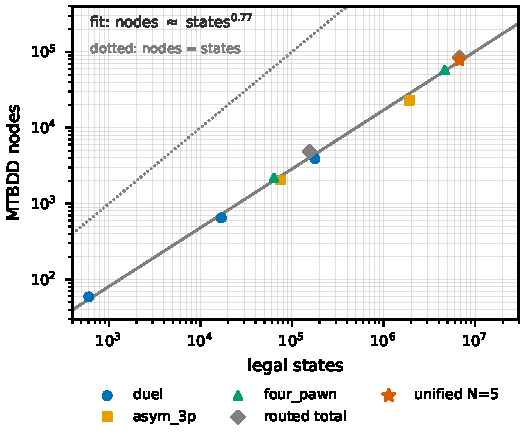
\includegraphics[width=\columnwidth]{figures/f1_growth.pdf}
\caption{MTBDD nodes vs.\ legal states, log-log (\tierm{}; compression\_summary.json).
All family builds, routed totals, and the unified $N{=}5$ build sit on a
sub-linear trend (pooled OLS exponent $0.775$; dotted line: nodes $=$ states).}
\label{fig:growth}
\end{figure}

\begin{figure}[t]
\centering
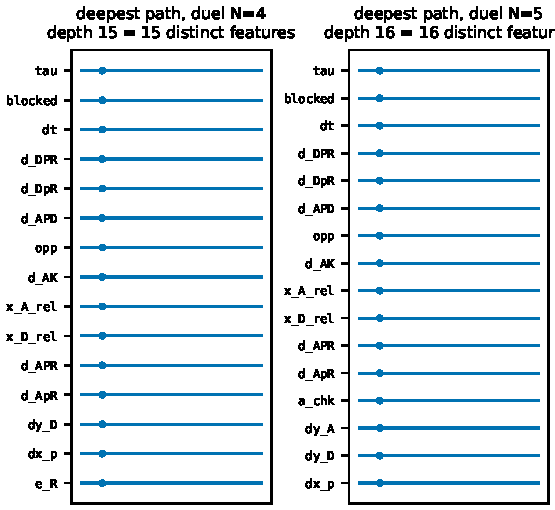
\includegraphics[width=\columnwidth]{figures/f4_paths.pdf}
\caption{Deepest root-to-leaf path of the duel MTBDD at $N{=}4$ (15 tests)
and $N{=}5$ (16 tests), with the feature tested at each level (\tierm{};
e3\_trace\_comparison.json). On an ordered MTBDD each feature appears at
most once per path, so depth $=$ distinct-feature count; board size adds
one new discriminating feature, not a proportional growth in tests.}
\label{fig:paths}
\end{figure}

\subsection{Growth law}
Pooling the ten family/total builds ($N\in\{3,4,5\}$, both build modes) and
fitting $\log_{10}(\text{nodes})$ on $\log_{10}(\text{states})$ by ordinary
least squares yields an exponent $k=0.775$ ($k=0.745$--$0.763$ within
families; Fig.~\ref{fig:growth}). Node counts grow meaningfully slower than
the state space: the $43.5\times$ state growth from $N{=}4$ to $N{=}5$
costs a $17.3\times$ routed node growth ($4{,}885\to84{,}618$; per-family
$6.0\times$, $11.2\times$, $26.4\times$), while the unified $N{=}5$ build
needs $78{,}305$ nodes ($16.0\times$ the routed $N{=}4$ total---a quotient
that crosses build modes and is quoted only for reference). The
consistent per-family range and the stable depth growth support a
sub-linear growth law over the measured range; we extrapolate no further
than $N{=}5$ except for the explicit $N{=}6$ depth prediction reported in
the companion diagnostics ($29$--$31$ plies, point estimate $30$, marked
\tiere{}).

\section{The Balance Axis (K2P+N)}
\label{sec:balance}

\subsection{Class selection and coverage}
Table~\ref{tab:classes} lists the seven class runs. Classes were chosen to
isolate the two candidate drivers of degradation: piece count (one added
knight per side at \emph{fixed} material balance) and material balance
(symmetric vs.\ unbalanced material at similar piece counts).

\begin{table*}[t]
\caption{K2P+N class-by-class compression (\tierm{}; class\_compression/*.json).
Ratio = legal class states per MTBDD node; verify = emitted-evaluator check
against the class oracle (0 value mismatches everywhere). RSS = peak MiB.}
\label{tab:classes}
\centering
\footnotesize
\begin{tabular}{llrrrrrrl}
\toprule
class (per side) & $N$ & states & orbits & nodes & depth & ratio & verify & RSS \\
\midrule
K+N vs K+N      & 3 & 2{,}112 & 528 & 47 & 13 & 1:44.9 & PASS, 0 mism. & 36 \\
K+N vs K+N      & 4 & 46{,}384 & 11{,}596 & 78 & 17 & 1:594.7 & PASS, 0 mism. & 56 \\
K+N vs K+N      & 5 & 391{,}072 & 97{,}804 & 139 & 16 & 1:2{,}813.5 & PASS, 0 mism. & 224 \\
K+P+N vs K      & 4 & 25{,}178 & 12{,}589 & 2{,}324 & 18 & 1:10.8 & PASS, 0 mism. & 67 \\
K+P+N vs K      & 5 & 249{,}728 & 124{,}912 & 11{,}252 & 21 & 1:22.2 & PASS, 0 mism. & 346 \\
K+P vs K+P+N    & 4 & 136{,}068 & 68{,}034 & 15{,}628 & 24 & 1:8.7 & PASS, 0 mism. & 213 \\
K+P+N vs K+P+N  & 4 & 1{,}358{,}808 & 339{,}702 & 73{,}013 & 28 & 1:18.6 & PASS (in-proc), 0 mism. & 814 \\
\bottomrule
\end{tabular}
\end{table*}

\subsection{Measured degradation}
The informative comparison is at fixed board size $N{=}4$, against the
knight-free K2P families built by the same pipeline:
\begin{itemize}
\item \textbf{Symmetric material:} K2P four\_pawn (K+2P vs K+2P, balanced)
compresses at 1:29.1; adding one knight per side at the same balance
(K+P+N vs K+P+N) compresses at 1:18.6---a $1.57\times$ degradation
(nodes 2{,}183$\to$73{,}013, depth 21$\to$28).
\item \textbf{Unbalanced material:} K2P asym\_3p (K+2P vs K+P) compresses at
1:36.3; adding a knight to the weaker side (K+P+N vs K) compresses at
1:10.8---a $3.35\times$ degradation. The mirror class (K+P vs K+P+N) is
worse still at 1:8.7.
\item \textbf{Knight-only classes:} K+N vs K+N compresses at 1:595--1:2{,}814.
These classes are draw-saturated with max DTC $=1$ (every decided state
converts immediately), so their ratios reflect a trivially simple value
structure; we exclude them from degradation claims rather than present them
as compression successes.
\end{itemize}
Every run's emitted evaluator verifies against its oracle with zero value
mismatches, and peak RSS stays below 814 MiB. Correctness is never traded
for compression: where the semantic basis cannot separate values, the
compiler pays in nodes and a conditional coordinate tail, not in errors.

\subsection{The balance reframe}
\label{sec:reframe}
We originally interpreted the degradation as a piece-count effect (``board
size helps, piece count hurts''). The measured class pattern supports a
different reading. First, at fixed balance, adding a knight per side costs
$1.57\times$---real, but modest. Second, at comparable piece counts,
unbalanced material costs far more: K+P+N vs K (3 pieces vs.\ 1) degrades
$3.35\times$ and K+P vs K+P+N $4.17\times$, versus $1.57\times$ for the
balanced K+P+N vs K+P+N. Third, depth grows most in the unbalanced classes
(24--28 vs.\ 21 at baseline), indicating more \emph{distinct} features in
play, not merely more states. We therefore revise the reading to:
\emph{material balance is the operative variable}; piece count contributes,
but balance amplifies the cost. The board-size axis helps precisely because
it does not touch balance or the feature basis; the balance axis hurts
because each imbalance injects new asymmetric structure (kings defending
different material) that the translation-invariant, symmetry-quotient
architecture cannot amortize. A fixed balance, growing pieces is the mild
case; imbalance is the hard case.

\begin{figure}[t]
\centering
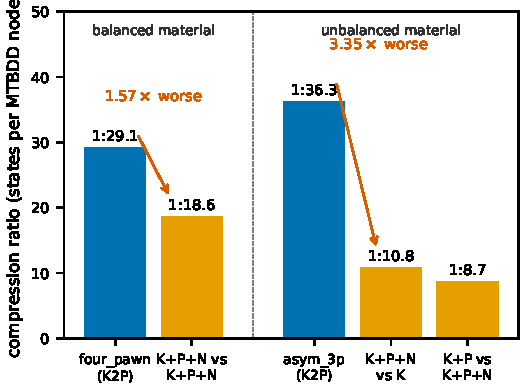
\includegraphics[width=\columnwidth]{figures/f2_degradation.pdf}
\caption{Compression ratio by material (\tierm{}; class\_compression/*.json).
Balanced material: K2P four\_pawn vs.\ K2P+N ($1.57\times$ degradation).
Unbalanced material: K2P asym\_3p vs.\ K+P+N vs K and K+P vs K+P+N
($3.35\times$ / $4.17\times$). Knight-only classes (1:595--1:2{,}814,
structurally trivial) are omitted from the bars.}
\label{fig:degradation}
\end{figure}
\section{Symbolic Certification (Z3)}
\label{sec:z3}

\subsection{The injectivity problem}
The compiler replaces states by feature vectors: two states with the same
feature vector $\varphi(s)$ are compiled into the same MTBDD leaf. This is
sound iff the basis is \emph{value-sufficient} on the class:
\begin{equation}
\forall s_1, s_2 \in C:\ \varphi(s_1) = \varphi(s_2) \Rightarrow
\mathrm{VAL}(s_1) = \mathrm{VAL}(s_2).
\label{eq:inj}
\end{equation}
When (\ref{eq:inj}) fails, the pipeline appends a conditional coordinate
tail (which restores exactness at node cost); when it holds, the semantic
basis alone suffices. Value-sufficiency is the precondition for tail-free
compilation; it is sufficient but not necessary for correct compilation, and
it says nothing about ratios.

\subsection{v1 refutation}
Basis v1 (5 king features + 13 knight features, plus 14 pawn features on
pawn classes; 18 features on knight classes, 32 on pawn classes) was tested
on all seven classes. The query ``$\exists s_1 s_2$: (\ref{eq:inj}) is
violated'' is \textsc{sat} on \emph{every} class: 4, 6, 6, 518, 4{,}004,
2{,}946, and 17{,}892 conflict buckets respectively, with Z3-certified
concrete counterexamples on the six classes that publish pairs; the mirror
class's refutation is carried by its 2{,}946 empirical conflict buckets
together with the symmetry proof and cross-oracle check of
\S\ref{sec:mirror} (Table~\ref{tab:z3}). Three ambiguity
mechanisms account for all counterexamples:
(1)~\emph{knight-square ambiguity}---positions differing only in the
knight's exact square share every distance feature (Chebyshev norms discard
direction) yet differ in mate-net geometry, hence in value;
(2)~\emph{rank-translation ambiguity}---whole positions shifted along a file
share all signed relative geometry but differ in edge-dependent mates;
(3)~\emph{pawn-geometry ambiguity}---same-distance, different-file pawn
placements relative to kings and knight.
The companion methodology paper in this repository (\texttt{paper/verification})
decodes a certified knight-square pair in detail.

\subsection{v2 fix and the minimality ladder}
Basis v2 adds eight signed knight offsets (per-axis deltas from each knight
to its own and the enemy king; $-1,-1$ when the piece is absent), two king
rank-edge distances ($\min(y, N{-}1{-}y)$), and, on pawn classes, eight
signed pawn offsets---28 features on knight classes, 50 on pawn classes.
With v2, the query is \textsc{unsat} on all seven classes: zero conflict
buckets (Table~\ref{tab:z3}). The signed offsets alone were
\emph{not} the fix---a minimality ladder of feature subsets, probed
empirically over the full classes, shows that knight-only classes require a
signed-offset family \emph{plus} the rank-edge pair, and pawn classes
require both signed-offset families plus signed pawn offsets
(Table~\ref{tab:ladder}); an opponent-orientation split changes nothing and
was dropped. The uniform v2 basis is therefore mildly overdetermined by
design: one class-independent definition rather than per-class minimality.

\begin{table}[t]
\caption{Z3 value-sufficiency before/after the basis repair (\tierm{};
z3\_injectivity\_v2.json). Conflicts = feature-equal buckets with differing
oracle values. Proofs: F = full-class unsat; S = bounded-subspace unsat
(fraction of class); E = empirical layer only (array axiomatisation skipped
above the 60{,}000-state cap).}
\label{tab:z3}
\centering
\footnotesize
\setlength{\tabcolsep}{3.2pt}
\begin{tabular}{lrrll}
\toprule
class & $N$ & v1 conf. & v2 conf. & proof (time) \\
\midrule
K+N vs K+N     & 3 & 4 & 0 & F, 1.7\,s \\
K+N vs K+N     & 4 & 6 & 0 & S (14.2\%), 2.5\,s \\
K+N vs K+N     & 5 & 6 & 0 & S (4.8\%), 18.7\,s \\
K+P+N vs K     & 4 & 518 & 0 & S (14.5\%), 1.9\,s \\
K+P+N vs K     & 5 & 4{,}004 & 0 & S (9.0\%), 22.8\,s \\
K+P vs K+P+N   & 4 & 2{,}946 & 0 & S (14.8\%), 18.8\,s \\
K+P+N vs K+P+N & 4 & 17{,}892 & 0 & E (1.36M states) \\
\bottomrule
\end{tabular}
\end{table}

\begin{table}[t]
\caption{Minimality ladder: conflict buckets under feature subsets
(\tierm{}; z3\_injectivity\_v2.json, minimality\_ladder). Shorthand:
kn = K+N vs K+N; kpn = K+P+N vs K; mirror = K+P vs K+P+N; both = K+P+N vs
K+P+N. A = knight$\to$own
signed offsets; B = knight$\to$enemy; C = king rank-edge distances;
D = pawn$\to$own signed offsets; E = pawn$\to$enemy; O = opp-orientation
split (redundant on every class, dropped).}
\label{tab:ladder}
\centering
\footnotesize
\setlength{\tabcolsep}{3pt}
\begin{tabular}{lrrrrrrr}
\toprule
class & v1 & A & B & AB & AB+C & AB+D & AB+E \\
\midrule
kn, $N{=}3$ & 4 & 4 & 4 & 8 & \textbf{0} & -- & -- \\
kn, $N{=}4$ & 6 & 8 & 8 & 8 & \textbf{0} & -- & -- \\
kn, $N{=}5$ & 6 & 16 & 8 & 8 & \textbf{0} & -- & -- \\
kpn, $N{=}4$ & 518 & 774 & 538 & 441 & -- & \textbf{0} & \textbf{0} \\
kpn, $N{=}5$ & 4{,}004 & 8{,}192 & 6{,}305 & 6{,}932 & -- & \textbf{0} & \textbf{0} \\
mirror, $N{=}4$ & 2{,}946 & 3{,}186 & 3{,}202 & 2{,}097 & -- & \textbf{0} & \textbf{0} \\
both, $N{=}4$ & 17{,}892 & 7{,}674 & 8{,}054 & 7{,}400 & -- & \textbf{0} & \textbf{0} \\
\bottomrule
\end{tabular}
\end{table}

\begin{figure}[t]
\centering
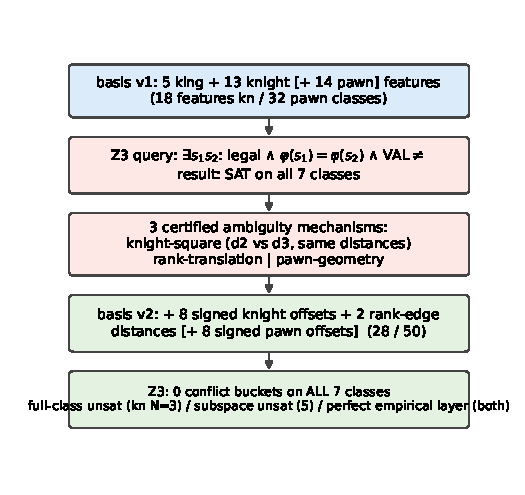
\includegraphics[width=\columnwidth]{figures/f3_z3_flow.pdf}
\caption{Certification flow: basis v1 is refuted on every class; three
certified ambiguity mechanisms motivate basis v2, which closes all seven
classes.}
\label{fig:z3flow}
\end{figure}

\subsection{Mirror symmetry}
For the K+P vs K+P+N class, Z3 proved---independently of VAL, in
0.25\,s---that $\varphi$ commutes with the colour-swap mirror $V'$
($\varphi(V'(s)) = \mathrm{swap}_{wb}(\varphi(s))$ with $\tau \to 1-\tau$;
the signed rank deltas are anti-invariant and negated under a piece-presence
guard). This is a property the \emph{v1} basis already had (unsat in
0.17\,s), so the basis repair preserved colour symmetry. As a semantic
cross-check, all 136{,}068 states of the class were re-evaluated under the
mirror against an \emph{independently solved} oracle (the K+P+N vs K+P+N
run): 0 mismatches.

\subsection{What Z3 proves and what it does not}
Z3 proves value-sufficiency of a feature basis on a (sub)space---a soundness
certificate for compilation. It does not prove optimality of the basis, does
not bound node counts, and does not transfer across material classes. On
five classes the proofs are bounded-subspace proofs (an array
axiomatisation over 3{,}640--22{,}375 states, 4.8--14.8\% of the class)
because the full-class axiomatisation exceeded the compute budget or the
60{,}000-state cap; on the 1.36M-state class only the empirical layer
(perfect injectivity over all 1{,}358{,}808 states) is available. The proof
tiers are reported per class rather than averaged into a headline.

\section{Connection to Balance Laws in the Literature}
\label{sec:balance-laws}
This section is discussion, not a primary contribution. Independent analyses
conducted outside this project (one using the Z.ai GLM model, one using
Google Gemini; attributed and marked non-peer-reviewed in the companion
repository's \textsc{supplementary/ai\_analyses.md}) arrive, from different
starting points, at a qualitative ``balance law'': the structural complexity
of pawn-endgame value functions concentrates where material is balanced.
Our class-by-class data are consistent with that claim---unbalanced classes
degrade $3.35\times$--$4.17\times$ versus $1.57\times$ for the balanced
class---and the balance reframe of \S\ref{sec:reframe} was made \emph{after}
the measurements. We do not claim to have proven any balance law; we claim
to have measured one instance of the pattern it predicts, on one fragment
family, with exact values.

\section{Discussion}
\label{sec:discussion}

\subsection{Why compression degrades at balance}
The structural reason is visible in the pipeline's own accounting. The orbit
quotient merges states that differ by colour-swap or board reflection; it
amortizes \emph{symmetric} structure. Board growth feeds the quotient
exponentially more states sharing the same relative geometry
(\S\ref{sec:board}). Material imbalance does the opposite: the sides'
kings assume qualitatively different roles (attacker vs.\ defender), the
role-assignment features split, and the number of distinct feature vectors
grows faster than the quotient can merge them---visible directly in the
conflicting-group counts (e.g., K+P+N vs K: 477 conflicting semantic groups
at $N{=}4$) and in depth growth (24--28 vs.\ 21). Balance, not piece count,
is what the architecture cannot amortize.

\subsection{What would extend this work}
Three extensions follow directly. (i)~\emph{K2P+R}: a sliding piece breaks
translation-invariance assumptions hardest and is the sharpest stress test
of the balance wall; it is proposed, not run. (ii)~\emph{Full K2P+N}: a
single workstation build ($\sim$17M states, $\sim$6\,GB peak RSS by the
measured per-state scaling) would replace the extrapolated full-space ratio
with one measured row. (iii)~\emph{Formal verification at scale}: the
subspace-proof boundary (\S\ref{sec:z3}) is an engineering budget, not a
mathematical one; a Lean formalization of the encoding would make the
certification total.

\subsection{What we are not claiming}
We are not claiming progress on the full game: the $8\times8$ initial
position is at the balance extreme, where this architecture is expected to
fare worst, and no measurement here contradicts the classical exponential
bounds \cite{fraenkel1983}. We are not claiming a novel decision diagram:
the MTBDD machinery is standard \cite{bryant1986,bahar1997,fujita1997}; the
contribution is the measurement discipline and the certification layer.

\section{Limitations and Non-Claims}
\label{sec:limits}
\textbf{Speed.} The emitted evaluator is \emph{slower} than a dictionary
lookup: 4.73 vs.\ 3.05\,\textmu s/state on the four\_pawn family (routed
full space 4.45\,\textmu s/state; CPython~3.12, best-of-passes, frozen-repo
benchmark). The contribution is verifiability---a pure-integer evaluator
whose every branch can be audited against the oracle---not speed.
\textbf{Extrapolations.} The full K2P+N $4\times4$ ratio ($\sim$1:20--25)
is extrapolated from the pawn-bearing class band (1:8.7--1:22.2) and is not
measured; the $N{=}6$ depth prediction (29--31) is a trend estimate. Both
are tagged \tiere{} in \textsc{facts.md}.
\textbf{Lost artifacts.} A sandbox outage destroyed the phase-level timing
split (E5) and the tuning result tables (Tracks A--D); both are reported as
lost, with the surviving walls and the charter's qualitative conclusions
(baseline variable ordering wins on nodes; unified emission saves
$\sim$7.5\% of nodes) cited instead. Nothing was reconstructed to fill the
gap.
\textbf{Proof coverage.} Five of seven Z3 verdicts rest on bounded subspaces
and one on the empirical layer alone; the certification is a budget-bounded
certificate, not a total proof.
\textbf{No theorem.} The balance-law reading is a measured pattern on one
family, not a theorem; no claim of generalization beyond K2P(+N) is made.
\textbf{No Lean verification.} The retrograde recursion itself is
empirically validated (self-tests, cross-checks, exhaustive verification),
not formally verified.

\section{Conclusion}
Across two independent scaling axes of a solved chess fragment, the same
compression architecture moves in opposite directions. Board size helps:
nodes grow as states$^{0.775}$, MTBDD depth grows by one to three tests
per step of $N$, and the
routed ratio improves from 1:31.7 to 1:79.7 (1:86.1 unified) from $N{=}4$
to $N{=}5$. Material balance hurts: $1.57\times$ at fixed balance,
$3.35\times$--$4.17\times$ unbalanced, with the worst measured class at
1:8.7. The architecture stays exact everywhere (0 mismatches on every
emitted evaluator), Z3 certifies the feature basis on all seven classes
after a signed-offset repair, and the balance reframe---balance, not piece
count, is the operative variable---is a measurement-supported revision, not
a fitted story. The piece-count wall documented here is a real boundary of
semantic-feature compression, and the two-axis method---solve, compile,
certify, measure, per class---is the transferable part.

\section*{Acknowledgment}
The author thanks the Z.ai and Google Gemini analyses for the independent
balance-law observations cited as non-peer-reviewed context in
\S\ref{sec:balance-laws}, and the Z3 team \cite{demoura2008} for the solver
this certification layer relies on.

\appendices
\section{Artifact and Reproducibility Statement}
All measurements in this paper resolve to JSON artifacts committed in the
companion repository \texttt{chess-compression-scaling}, whose
\textsc{facts.md} (88 rows, generated programmatically from those artifacts)
lists every claim with its exact file and key path; the paper cites the
\textsc{measured} subset. The source solver and compressor are the
unmodified scripts of the frozen K2P artifact \cite{k2p2025} (commit
\texttt{76ba614}); the $N$-parameterized oracle/compressor and the class and
certification scripts live under \texttt{experiments/} in the companion
repository. The trust gates of \S\ref{sec:gates} are re-runnable in
minutes: the $N{=}4$ oracle solves in $\sim$2\,s and the $N{=}4$ compression
of all three families reproduces the 4{,}885-node routed total; a CI workflow
runs this gate on every push. The $N{=}5$ oracle solve is $\sim$110\,s wall
in the authoring sandbox (CPython 3.12, NumPy 2.1); the smallest Z3
certification (K+N vs K+N, $N{=}3$) re-runs in $\sim$1.7\,s on the released
per-class arrays. Two caveats are part of the record, not footnotes: the
phase-level timing split and the tuning-phase result tables were lost to a
sandbox outage and are reported as lost, and the full K2P+N $4\times4$ build
was deliberately not run, so the full-space K2P+N ratio remains an
extrapolation.

\bibliographystyle{IEEEtran}
\bibliography{refs}

\end{document}
